%% ============================================================
%%  Distributed IoT Stock Tracking System — Project Summary
%%  Author  : Alper
%%  Date    : April 2026
%%  Engine  : pdfLaTeX
%%  Purpose : ~5-page executive summary of the full project
%% ============================================================
\documentclass[11pt,a4paper]{article}

%% ---- Encoding & Language ----
\usepackage[utf8]{inputenc}
\usepackage[T1]{fontenc}
\usepackage[english]{babel}

%% ---- Typography ----
\usepackage{lmodern}
\usepackage{microtype}
\usepackage{setspace}
\onehalfspacing

%% ---- Page Geometry ----
\usepackage[
  a4paper,
  top=2.2cm, bottom=2.2cm,
  left=2.8cm, right=2.5cm
]{geometry}

%% ---- Headers ----
\usepackage{fancyhdr}
\pagestyle{fancy}
\fancyhf{}
\fancyhead[L]{\small\textit{Distributed IoT Stock Tracking System --- Project Summary}}
\fancyhead[R]{\small\thepage}
\renewcommand{\headrulewidth}{0.4pt}

%% ---- Color ----
\usepackage{xcolor}
\definecolor{primary}{HTML}{1565C0}
\definecolor{secondary}{HTML}{0288D1}
\definecolor{accent}{HTML}{00ACC1}
\definecolor{success}{HTML}{2E7D32}
\definecolor{danger}{HTML}{C62828}
\definecolor{warning}{HTML}{E65100}
\definecolor{neutral}{HTML}{546E7A}
\definecolor{codebg}{HTML}{F5F5F5}
\definecolor{codeframe}{HTML}{CCCCCC}
\definecolor{keyword}{HTML}{0033B3}
\definecolor{string}{HTML}{067D17}
\definecolor{comment}{HTML}{8C8C8C}

%% ---- Listings ----
\usepackage{listings}
\usepackage{lstautogobble}
\lstdefinestyle{plain}{
  backgroundcolor=\color{codebg},
  frame=single, rulecolor=\color{codeframe},
  basicstyle=\ttfamily\small,
  keywordstyle=\color{keyword}\bfseries,
  stringstyle=\color{string},
  commentstyle=\color{comment}\itshape,
  breaklines=true, autogobble=true,
  tabsize=2, numbers=none
}

%% ---- Tables ----
\usepackage{booktabs}
\usepackage{tabularx}
\usepackage{array}

%% ---- Graphics / TikZ ----
\usepackage{graphicx}
\usepackage{tikz}
\usetikzlibrary{
  shapes.geometric, arrows.meta, positioning,
  fit, backgrounds, calc, shadows
}

\tikzset{
  box/.style={
    rectangle, rounded corners=4pt, draw=#1!75!black,
    fill=#1!18, text centered, font=\small\bfseries,
    minimum height=0.75cm, minimum width=2.2cm,
    drop shadow={shadow xshift=0.8pt, shadow yshift=-0.8pt,
                 fill=#1!50!black, opacity=0.25}
  },
  arr/.style={-Stealth, thick, draw=neutral!65},
  grp/.style={rectangle, rounded corners=5pt,
              draw=neutral!50, fill=neutral!5, inner sep=7pt}
}

%% ---- Misc ----
\usepackage{enumitem}
\usepackage{float}
\usepackage{caption}
\usepackage{mdframed}
\captionsetup{font=small, labelfont=bf, margin=0.4cm}
\usepackage[
  colorlinks=true, linkcolor=black,
  citecolor=blue!65!black, urlcolor=blue!65!black,
  pdftitle={Distributed IoT Stock Tracking — Project Summary},
  pdfauthor={Alper}
]{hyperref}

%% ---- Custom commands ----
\newcommand{\tech}[1]{\textit{#1}}
\newcommand{\pkg}[1]{\texttt{#1}}
\newcommand{\hdr}[1]{\vspace{4pt}\noindent\textcolor{primary}{\textbf{#1}}\quad}

%% ============================================================
\begin{document}

%% ---- Title ----
\begin{center}
  {\LARGE\bfseries\color{primary}
    Distributed IoT Stock Tracking System}\\[0.5em]
  {\large\color{secondary}
    Project Summary}\\[0.3em]
  {\normalsize Alper \quad|\quad April 2026}
  \vspace{0.4em}
  \hrule height 1.2pt
\end{center}

\vspace{0.4em}

%% ============================================================
\section*{1.\quad Overview}
%% ============================================================

This project implements a \textbf{production-like distributed stock-tracking
platform} whose primary objective is to make the trade-offs of the
\emph{CAP Theorem} (Brewer, 2000) observable and measurable through live
fault injection.

The system is built around a \tech{Spring Boot 3.x} backend, a
\tech{Kafka 4.1} event bus, a \tech{Redis 7} cache, a \tech{MySQL 8}
relational database, a \tech{Python 3.11} IoT sensor simulator, and a
\tech{React 18} single-page application.
All eleven services are containerised and orchestrated with
\tech{Docker Compose}.
\tech{Toxiproxy} sits transparently in front of every infrastructure
component so that network partitions can be injected and removed on demand
via a REST API.

\vspace{0.3em}

\begin{mdframed}[backgroundcolor=primary!5, linecolor=primary!40, linewidth=0.8pt]
\small
\textbf{Key delivery guarantees:}\\
\textbullet\; \emph{At-least-once} Kafka event delivery via the Transactional Outbox Pattern.\\
\textbullet\; \emph{Full functional availability} during Redis or Kafka partitions.\\
\textbullet\; \emph{Hard fail-fast} (HTTP 500) only on MySQL partition --- no
              safe fallback exists for the source of truth.
\end{mdframed}

%% ============================================================
\section*{2.\quad Architecture}
%% ============================================================

Figure~\ref{fig:arch} shows the three-layer topology.
Table~\ref{tab:services} lists all Docker services.

\begin{figure}[H]
\centering
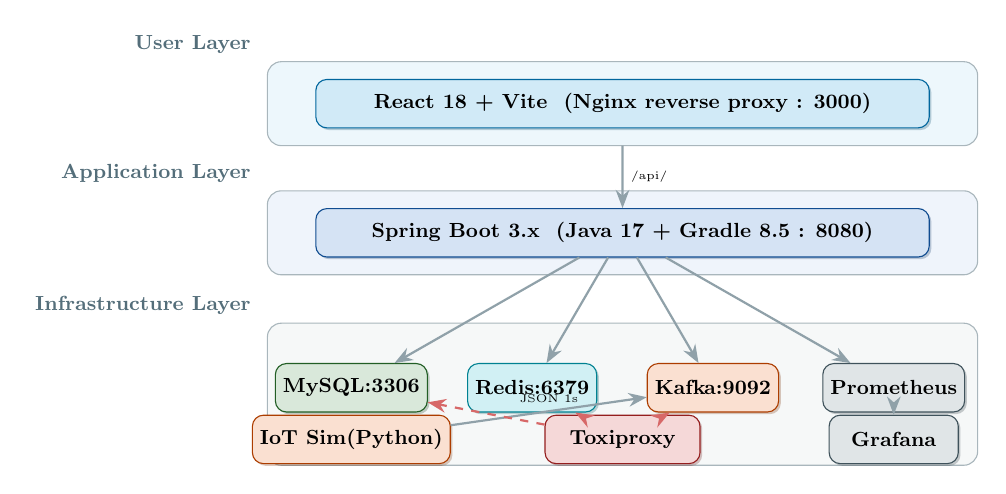
\begin{tikzpicture}[node distance=0.5cm, scale=0.82, every node/.style={scale=0.82}]

  %% User layer
  \begin{scope}[on background layer]
    \node[grp, minimum width=11cm, minimum height=1.3cm, fill=secondary!7]
      (ul) at (0,0) {};
  \end{scope}
  \node[font=\bfseries\small, text=neutral, above left=0pt and 3pt of ul.north west]
    {User Layer};
  \node[box=secondary, minimum width=9.5cm] at (0,0)
    {React 18 + Vite\ \ (Nginx reverse proxy : 3000)};

  %% Application layer
  \begin{scope}[on background layer]
    \node[grp, minimum width=11cm, minimum height=1.3cm, fill=primary!7]
      (al) at (0,-2.0) {};
  \end{scope}
  \node[font=\bfseries\small, text=neutral, above left=0pt and 3pt of al.north west]
    {Application Layer};
  \node[box=primary, minimum width=9.5cm] (be) at (0,-2.0)
    {Spring Boot 3.x\ \ (Java 17 + Gradle 8.5 : 8080)};

  %% Infrastructure layer
  \begin{scope}[on background layer]
    \node[grp, minimum width=11cm, minimum height=2.2cm, fill=neutral!5]
      (il) at (0,-4.5) {};
  \end{scope}
  \node[font=\bfseries\small, text=neutral, above left=0pt and 3pt of il.north west]
    {Infrastructure Layer};

  \node[box=success, minimum width=2.0cm] (mysql) at (-4.2,-4.4)  {MySQL\\:3306};
  \node[box=accent,  minimum width=2.0cm] (redis) at (-1.4,-4.4)  {Redis\\:6379};
  \node[box=warning, minimum width=2.0cm] (kafka) at (1.4,-4.4)   {Kafka\\:9092};
  \node[box=neutral, minimum width=2.0cm] (prom)  at (4.2,-4.4)   {Prometheus};
  \node[box=neutral, minimum width=2.0cm] (graf)  at (4.2,-5.2)   {Grafana};
  \node[box=danger,  minimum width=2.4cm] (toxi)  at (0,-5.2)     {Toxiproxy};
  \node[box=warning, minimum width=2.0cm] (iot)   at (-4.2,-5.2)  {IoT Sim\\(Python)};

  \draw[arr] (0,-0.65) -- node[right,font=\tiny]{/api/} (be);
  \draw[arr] (be) -- (mysql); \draw[arr] (be) -- (redis);
  \draw[arr] (be) -- (kafka); \draw[arr] (be) -- (prom);
  \draw[arr] (prom) -- (graf);
  \draw[arr] (iot) -- node[above,font=\tiny]{JSON 1s} (kafka);
  \draw[arr, dashed, draw=danger!70] (toxi) -- (mysql);
  \draw[arr, dashed, draw=danger!70] (toxi) -- (redis);
  \draw[arr, dashed, draw=danger!70] (toxi) -- (kafka);

\end{tikzpicture}
\caption{Three-layer architecture. Dashed red lines = Toxiproxy fault injection paths.}
\label{fig:arch}
\end{figure}

\begin{table}[H]
\centering
\caption{Docker Compose service inventory (11 containers)}
\label{tab:services}
\small
\begin{tabularx}{\textwidth}{@{}llX@{}}
\toprule
\textbf{Container} & \textbf{Port(s)} & \textbf{Role} \\
\midrule
\texttt{stock-app}      & 8080        & Spring Boot REST API + SSE \\
\texttt{stock-frontend} & 3000        & React SPA inside Nginx reverse proxy \\
\texttt{iot-simulator}  & ---         & Python temperature sensor (1 msg/s) \\
\texttt{mysql-db}       & 3306        & Source of truth + Outbox table \\
\texttt{redis-master}   & 6379        & Cache R/W + sensor data store \\
\texttt{redis-replica}  & 6380        & Read-only standby \\
\texttt{kafka-kraft}    & 9092        & Event bus (KRaft, no ZooKeeper) \\
\texttt{toxiproxy}      & 8474 / 3307 / 26379 / 29093 & Fault injection proxy \\
\texttt{prometheus}     & 9090        & Metrics scraping (15 s) \\
\texttt{grafana}        & 3001        & Stock + IoT dashboards \\
\bottomrule
\end{tabularx}
\end{table}

%% ============================================================
\section*{3.\quad Backend Domain Structure}
%% ============================================================

The Spring Boot application is organised into three \textbf{vertical domain
slices} rather than a horizontal technical-layer layout.
Each domain is self-contained; the \pkg{shared} package holds only
cross-cutting infrastructure.

\begin{lstlisting}[style=plain]
com.example.Thesis
|-- stock/          # Stock-tracking bounded context
|   |-- controller/ StockController, LoadTestController
|   |-- service/    StockService, KafkaProducerService
|   |-- outbox/     OutboxEvent, OutboxEventStatus, OutboxScheduler
|   |-- dto/        StockEventDto, StockRequestDto, StockResponseDto
|   |-- model/      Stock
|   +-- repository/ StockRepository, OutboxEventRepository
|
|-- sensor/         # IoT sensor bounded context
|   |-- controller/ SensorController (SSE + REST)
|   |-- listener/   SensorDataListener (KafkaListener)
|   +-- dto/        SensorDataDto (@JsonProperty wire mapping)
|
+-- shared/         # Cross-cutting infrastructure
    |-- cache/      CacheService (interface), RedisCacheService
    |-- config/     KafkaProducerConfig, KafkaConsumerConfig,
    |               RedisConfig, MetricsConfig, CorsConfig, WebMvcConfig
    +-- ratelimit/  RateLimitingService, RateLimitInterceptor
\end{lstlisting}

\noindent\textbf{Why domain slices?}
The \pkg{stock} and \pkg{sensor} packages share no direct class references.
This low coupling makes it straightforward to extract either domain
into an independent microservice without touching the other.

%% ============================================================
\section*{4.\quad Key Design Patterns}
%% ============================================================

\subsection*{4.1\quad Transactional Outbox}

Every stock mutation atomically writes both the record \emph{and} an
\texttt{outbox\_events} entry inside one \texttt{@Transactional} context.
An \texttt{OutboxScheduler} polls for \texttt{PENDING} events every 5 seconds
and forwards them to Kafka using a \emph{synchronous} send, enabling clear
retry semantics (max 5 attempts before marking \texttt{FAILED}).

\smallskip
\noindent\textbf{Result:} delivery guarantee upgraded from
\emph{at-most-once} to \emph{at-least-once} without any change to the
HTTP API contract.

\subsection*{4.2\quad Cache-Aside / Write-Through (Redis)}

On creation and update, Redis is populated immediately after the DB commit
(\emph{write-through}).
On a read, the service checks Redis first; a cache miss falls back to MySQL
and repopulates the cache (\emph{cache-aside}).
When Redis is partitioned, the exception is caught silently and MySQL is
queried directly --- no crash, no cache write to avoid stale entries.

\smallskip
\begin{center}
\small
\begin{tabular}{@{}lrr@{}}
\toprule
\textbf{Condition} & \textbf{GET latency} & \textbf{POST latency} \\
\midrule
Cache HIT (normal) & $<10$\,ms    & $\sim$80\,ms \\
Cache MISS (normal) & $\sim$50\,ms & $\sim$80\,ms \\
Redis partitioned & $\sim$5050\,ms & $\sim$85\,ms \\
\bottomrule
\end{tabular}
\end{center}

\subsection*{4.3\quad IoT Sensor Pipeline}

The Python simulator publishes one JSON reading per second to the
\texttt{warehouse-metrics} Kafka topic.
\texttt{SensorDataListener} consumes it, writes structured JSON to
Redis (\texttt{sensor:<deviceId>}, TTL 5 min), and raises a Redis List
alert when temperature exceeds 30\,\textdegree{}C.
\texttt{SensorController} exposes the data via \textbf{Server-Sent Events}
(SSE) so the React dashboard receives live updates without polling.

The DTO decouples the wire format from the domain:

\begin{lstlisting}[style=plain, language=Java]
public class SensorDataDto {
    @JsonProperty("cihazId")  private String deviceId;   // Turkish wire key
    @JsonProperty("sicaklik") private Double temperature;
    @JsonProperty("zaman")    private String timestamp;
}
\end{lstlisting}

\subsection*{4.4\quad Rate Limiting (Token Bucket)}

A Bucket4j interceptor enforces \textbf{50 req/s} on all \texttt{/api/**}
routes. Excess requests receive HTTP~429.

\subsection*{4.5\quad CAP Theorem Positioning}

\begin{center}
\small
\begin{tabular}{@{}llll@{}}
\toprule
\textbf{Component} & \textbf{CAP} & \textbf{On Partition} & \textbf{Strategy} \\
\midrule
MySQL  & CP & Fail $\to$ HTTP 500 & Fail-fast (no fallback) \\
Redis  & AP & Fail $\to$ DB fallback & Cache-aside graceful degrade \\
Kafka  & CP$\to$AP & Fail $\to$ Outbox queues & Retry via scheduler \\
\textit{System} & \textit{AP} & \multicolumn{2}{l}{\textit{Available under Redis \& Kafka partitions}} \\
\bottomrule
\end{tabular}
\end{center}

%% ============================================================
\section*{5.\quad Observability}
%% ============================================================

\hdr{Prometheus} scrapes \texttt{/actuator/prometheus} every 15 seconds.
Beyond JVM auto-instrumentation, 12 custom Micrometer metrics are defined:
cache hit/miss counters, Redis op timers, Kafka producer success/failure
counters, stock-operation timers, Outbox sent/failed/retried counters,
an Outbox pending gauge, and IoT sensor received/alert/error counters.

\hdr{Grafana} provisions two dashboards automatically:

\begin{enumerate}[noitemsep, leftmargin=1.5cm]
  \item \textbf{Stock Metrics} --- cache hit rate, Kafka throughput, HTTP rate,
        JVM heap, Redis reconnect count.
  \item \textbf{IoT Sensor Metrics} --- temperature time series, alert rate,
        consumer lag, partition health.
\end{enumerate}

%% ============================================================
\section*{6.\quad Refactoring Phase}
%% ============================================================

After the initial integration was complete, a targeted refactoring pass
corrected three architectural issues found during code review:

\begin{enumerate}[leftmargin=1.5cm, label=\textbf{R\arabic*.}]
  \item \textbf{Domain-slice package layout} (described in \S3).
        Replaced flat technical layers with bounded-context directories;
        37 files moved, all imports updated, \texttt{gradle build} verified
        green after each step.

  \item \textbf{Outbox bypass fix.}
        The original \texttt{StockService} called
        \texttt{kafkaProducerService.sendStockEvent()} directly --- a
        fire-and-forget async call that silently discarded events during
        Kafka outages. The \texttt{outbox\_events} table was never written to.
        Corrected by removing the direct Kafka call and writing the outbox
        entry inside the same transaction as the stock mutation.

  \item \textbf{Redis pipe-format to JSON.}
        \texttt{SensorDataListener} previously stored Redis values as
        custom pipe-delimited strings
        (\texttt{Temperature=24.5\textdegree{}C|Time=...}).
        \texttt{SensorController} parsed them with \texttt{split("|")}.
        Both classes now use \texttt{ObjectMapper} for structured,
        self-describing JSON serialisation.
\end{enumerate}

%% ============================================================
\section*{7.\quad CI/CD Pipeline}
%% ============================================================

A GitHub Actions workflow runs on every push to \texttt{master}/\texttt{main}:

\begin{enumerate}[noitemsep, leftmargin=1.5cm]
  \item Java build + JUnit tests (Gradle 8.5)
  \item React SPA build (\texttt{npm ci \&\& npm run build})
  \item Docker Buildx setup (fixes \emph{``Cache export not supported''} error)
  \item Three Docker image push to GitHub Container Registry:
        \texttt{thesis-app}, \texttt{thesis-frontend}, \texttt{thesis-iot-simulator}.
        Each tagged \texttt{latest} and \texttt{sha-\{commit\}}.
\end{enumerate}

%% ============================================================
\section*{8.\quad Performance Summary}
%% ============================================================

\begin{center}
\small
\begin{tabular}{@{}lrrll@{}}
\toprule
\textbf{Scenario} & \textbf{Throughput} & \textbf{Success} & \textbf{Notes} \\
\midrule
Normal (no toxic)       & 200 ops/s & 100\% & Baseline \\
Kafka 500 ms latency    & 125 ops/s & 100\% & 62.5\% of baseline \\
Kafka 2000 ms latency   &  25 ops/s & 100\% & Linear degradation \\
Kafka full partition     &   0 ops/s &   0\% & Events queued in Outbox \\
Redis partition          & 200 ops/s & 100\% & +5 s GET latency \\
\bottomrule
\end{tabular}
\end{center}

\noindent JVM heap stabilises at $\approx$40\,MB at 200\,ops/s.
Connection pools: 10 MySQL (HikariCP), async Lettuce (Redis),
5 in-flight Kafka producer requests.

%% ============================================================
\section*{9.\quad Technology Stack}
%% ============================================================

\begin{center}
\small
\begin{tabular}{@{}lll@{}}
\toprule
\textbf{Layer} & \textbf{Technology} & \textbf{Version} \\
\midrule
Language        & Java                & 17 \\
Framework       & Spring Boot         & 3.5.9 \\
Build           & Gradle              & 8.5 \\
Event Bus       & Apache Kafka (KRaft)& 4.1.1 \\
Cache           & Redis               & 7-alpine \\
Database        & MySQL               & 8.0 \\
Rate Limiter    & Bucket4j            & 8.10.1 \\
Metrics         & Micrometer + Prometheus & latest \\
Dashboards      & Grafana             & latest \\
Fault Injection & Toxiproxy (Shopify) & latest \\
Frontend        & React + Vite        & 18 / 6.x \\
IoT Simulator   & Python              & 3.11 \\
Container Proxy & Nginx               & alpine \\
\bottomrule
\end{tabular}
\end{center}

%% ============================================================
\section*{10.\quad Conclusion}
%% ============================================================

This project delivers a complete, working demonstration of CAP Theorem
trade-offs on a realistic workload.
The system remains fully available under Redis and Kafka partitions while
correctly failing fast under a MySQL partition.
The Transactional Outbox Pattern \emph{correctly wired} inside a shared
database transaction guarantees zero event loss during broker outages.
A domain-slice package refactoring and structured Redis serialisation
raise the codebase to professional maintainability standards,
making each bounded context independently evolvable.

\vspace{1em}
\begin{mdframed}[backgroundcolor=success!5, linecolor=success!40, linewidth=0.8pt]
\small\noindent
\textbf{Repository:}
\url{https://github.com/nothinglikeFreshWeather/Thesis}\\
\textbf{Container Registry:}
\texttt{ghcr.io/nothinglikefreshweather/thesis-\{app|frontend|iot-simulator\}}
\end{mdframed}

\end{document}
